\documentclass[12pt,a4paper]{article}

% To use this template make changes to following:
% 1. Fill-ables section.
% 2. Instructions.
% 3. Marks table.
% 4. Actual questions.

% ================================ 1. Fill-ables ================================
\newcommand\University{National University of Computer and Emerging Sciences}
\newcommand\Department{School of Engineering}
\newcommand\Campus{Islamabad Campus}
\newcommand\Semester{Summer 2014}
\newcommand\Exam{Final Exam}
\newcommand\Subject{EE308--Microwave Engineering}
\newcommand\ExamDate{Saturday, August 09, 2014}
\newcommand\InstructorOne{Attique Dawood}
\newcommand\InstructorTwo{}
\newcommand\InstructorThree{\null}
\newcommand\TotalTime{03 Hours}
\newcommand\TotalMarks{100}
\newcommand\TotalQuestions{5}
\newcommand\TotalPages{\pageref{LastPage}} % Automatic: No need to change this.
% Marks of each question
\def\Qone{20}
\def\Qtwo{20}
\def\Qthree{20}
\def\Qfour{20}
\def\Qfive{20}
\def\Qsix{0}
\def\Qseven{0}
\def\Qeight{0}
\def\Qnine{0}
\def\Qten{0}
% ============================================================================

% ============== 2. Packages ==============
\usepackage{amsmath}
\usepackage{float}
\usepackage{graphicx}
\usepackage[hyphens]{url}
\usepackage[hidelinks]{hyperref}	% Clickable links to figures, references and urls.
\usepackage{lastpage}
\usepackage{array}
\usepackage{fancyhdr}
\usepackage{afterpage}
% Drawing packages.
\usepackage{pgf}
\usepackage{tikz}
% Listings for formatting code.
\usepackage{listings}
\usepackage{textcomp}

% General listings options.
\lstset{breaklines=true, basicstyle=\footnotesize\ttfamily, tabsize=4, numbers=left, stepnumber=1, frame=none, showstringspaces=false, upquote=true}
% C++ specific high-lighting. Comments are 50/50 shades of green/black and strings coloured with 60/40 red/black mixture.
\lstset{language=[ISO]C++, commentstyle=\color{green!50!black}, keywordstyle=\color{blue}, stringstyle=\color{red!60!black}}

% Table cell alignment directives.
\newcolumntype{L}[1]{>{\raggedright\let\newline\\\arraybackslash\hspace{0pt}}m{#1}}
\newcolumntype{C}[1]{>{\centering\let\newline\\\arraybackslash\hspace{0pt}}m{#1}}
\newcolumntype{R}[1]{>{\raggedleft\let\newline\\\arraybackslash\hspace{0pt}}m{#1}}

% Line spacing.
\def\SingleSpacing{\def\baselinestretch{1}\large\normalsize}
\def\DoubleSpacing{\def\baselinestretch{1.5}\large\normalsize}

% Margins.
\setlength{\oddsidemargin}{0in}
\setlength{\evensidemargin}{0in}
\setlength{\headheight}{28pt}
\setlength{\headsep}{2.5pt}
\setlength{\topmargin}{-60pt}
\setlength{\textwidth}{6.5in}
\setlength{\textheight}{10.75in} % Actual: 10.75in

% ============================= 3. Header and Footer ============================
\pagestyle{empty}
% Header
\chead
{
	{\large\textbf{\University}}\\
	\begin{minipage}{0.45\textwidth}
	\begin{center}
	{\small\textbf{\Department}}
	\end{center}
	\end{minipage}
	\begin{minipage}{0.45\textwidth}
	\begin{center}
	{\small\textbf{\Campus}}
	\end{center}
	\end{minipage}
}
% Footer
\lfoot{{\small\Exam}}
\cfoot{{\small\Semester}}
\rfoot{{\small Page \textbf{\thepage}~of \textbf{\TotalPages}}}
\renewcommand{\headrulewidth}{0.4pt}
\renewcommand{\footrulewidth}{0.4pt}
% ================================= 4. Front Page ===============================
\begin{document}
% A cute macro to add up marks of all individual questions. Uncomment if you want to use this.
\pgfmathtruncatemacro\TotalMarks{\Qone+\Qtwo+\Qthree+\Qfour+\Qfive+\Qsix+\Qseven+\Qeight+\Qnine+\Qten}
% Use this macro if marks are in decimal points
%\newcommand\TotalMarks{\pgfmathsetmacro\TotalMarks{\Qone+\Qtwo+\Qthree+\Qfour+\Qfive+\Qsix+\Qseven+\Qeight+\Qnine+\Qten}}
\begin{minipage}[t]{0.6\textwidth}
\begin{flushleft}
\DoubleSpacing
{\Large\textbf{\Subject}}\\
{\normalsize\ExamDate}\\
{\large\textbf{Course Instructor}}\\
{\normalsize\InstructorOne}\\
{\normalsize\InstructorTwo}
{\normalsize\InstructorThree}
\end{flushleft}
\end{minipage}
\begin{minipage}[t]{0.01\textwidth}
~
\end{minipage}
\begin{minipage}[t]{0.325\textwidth}
\DoubleSpacing
{\normalsize Serial No:}\\
{\Large\textbf{\Exam}}\\
{\large\textbf{Total Time: \TotalTime}}\\
{\large\textbf{Total Marks: \TotalMarks}}\\[1cm]
\rule{5cm}{0.2mm}\\[-0.25cm]
{\small Signature of Invigilator}
\end{minipage}
\SingleSpacing
~\\[1.5cm] % Extra space.
\rule{7cm}{0.2mm}~\rule{2.5cm}{0.2mm}~\rule{2cm}{0.2mm}~\rule{4.5cm}{0.2mm}\\
{\small Student Name\hspace{4.75cm}Roll No\hspace{1.35cm}Section\hspace{0.95cm}Signature}\\[1cm]
% ============================ 5. Instructions ==================================
\textbf{DO NOT OPEN THE QUESTION BOOK OR START UNTIL INSTRUCTED.}\\
\textbf{Instructions:}
\begin{enumerate}
\itemsep0em
\item Verify at the start of the exam that you have a total of \TotalQuestions~questions printed on \TotalPages~pages including this title page.
\item Attempt all questions on the question-book and in the given order.
\item The exam is closed books, closed notes. Please see that the area in your threshold is free of any material classified as `useful in the paper' or else there may be a charge of cheating.
\item Read the questions carefully for clarity of context and understanding of meaning and make assumptions wherever required, for neither the invigilator will address your queries, nor the teacher/examiner will come to the examination hall for any assistance.
\item Fit in all your answers in the provided space. You may use extra space on the last page if required. If you do so, clearly mark question/part number on that page to avoid confusion. 
\item Use only your own stationery and calculator. If you do not have your own calculator, use manual calculations. 
\item Use only permanent ink-pens. Only the questions attempted with permanent ink-pens will be considered. Any part of paper done in lead pencil cannot be claimed for checking/rechecking.
\end{enumerate}
% =============================== 6. Marks Table ================================
\begin{table}[H]
\begin{center}
\vspace{0.3cm}
	{\footnotesize \begin{tabular}{|C{1.8cm}|C{0.75cm}|C{0.75cm}|C{0.75cm}|C{0.75cm}|C{0.75cm}|c|}
	\hline
		\rule{0pt}{4.6ex} & Q-1 & Q-2 & Q-3 & Q-4 & Q-5 & \textbf{Total}\\[-0.5ex]
		\hline
		\rule{0pt}{2.5ex}\textbf{Total Marks}& \Qone & \Qtwo & \Qthree & \Qfour & \Qfive & \TotalMarks\\
		\hline
		\rule{0pt}{2.5ex}\textbf{Marks Obtained}& & & & & &\\
	\hline
	\end{tabular}}
\end{center}
\end{table}
{\small \textbf{Vetted By: \rule{6cm}{0.2mm} Vetter Signature: \rule{4.5cm}{0.2mm}}}
\setlength{\textheight}{10.5in}
\newpage
\pagestyle{fancy}
% ================================== 7. Questions ===============================
\noindent\textbf{Question 1: \hfill \Qone~marks}\\
A $75+j40\Omega$ load is connected to a $50\Omega$ transmission line. Use manual calculations to find,
\begin{itemize}
\item[a.] $\Gamma$
\item[b.] VSWR
\item[c.] $Z_{in}$ at $0.3\lambda$ from load
\item[d.] $Z_{in}$ at generator if line is $0.6\lambda$ long.
\end{itemize}
\newpage
\noindent \textbf{Question 2: \hfill \Qtwo~marks}\\
Repeat Question 1 using Smith Chart. Also, find values of $V_{max}$ and $V_{min}$ in addition to their locations on the line.
\newpage
\begin{figure}[H]
\centering
\vspace{4cm}
\hspace*{-1.6cm}
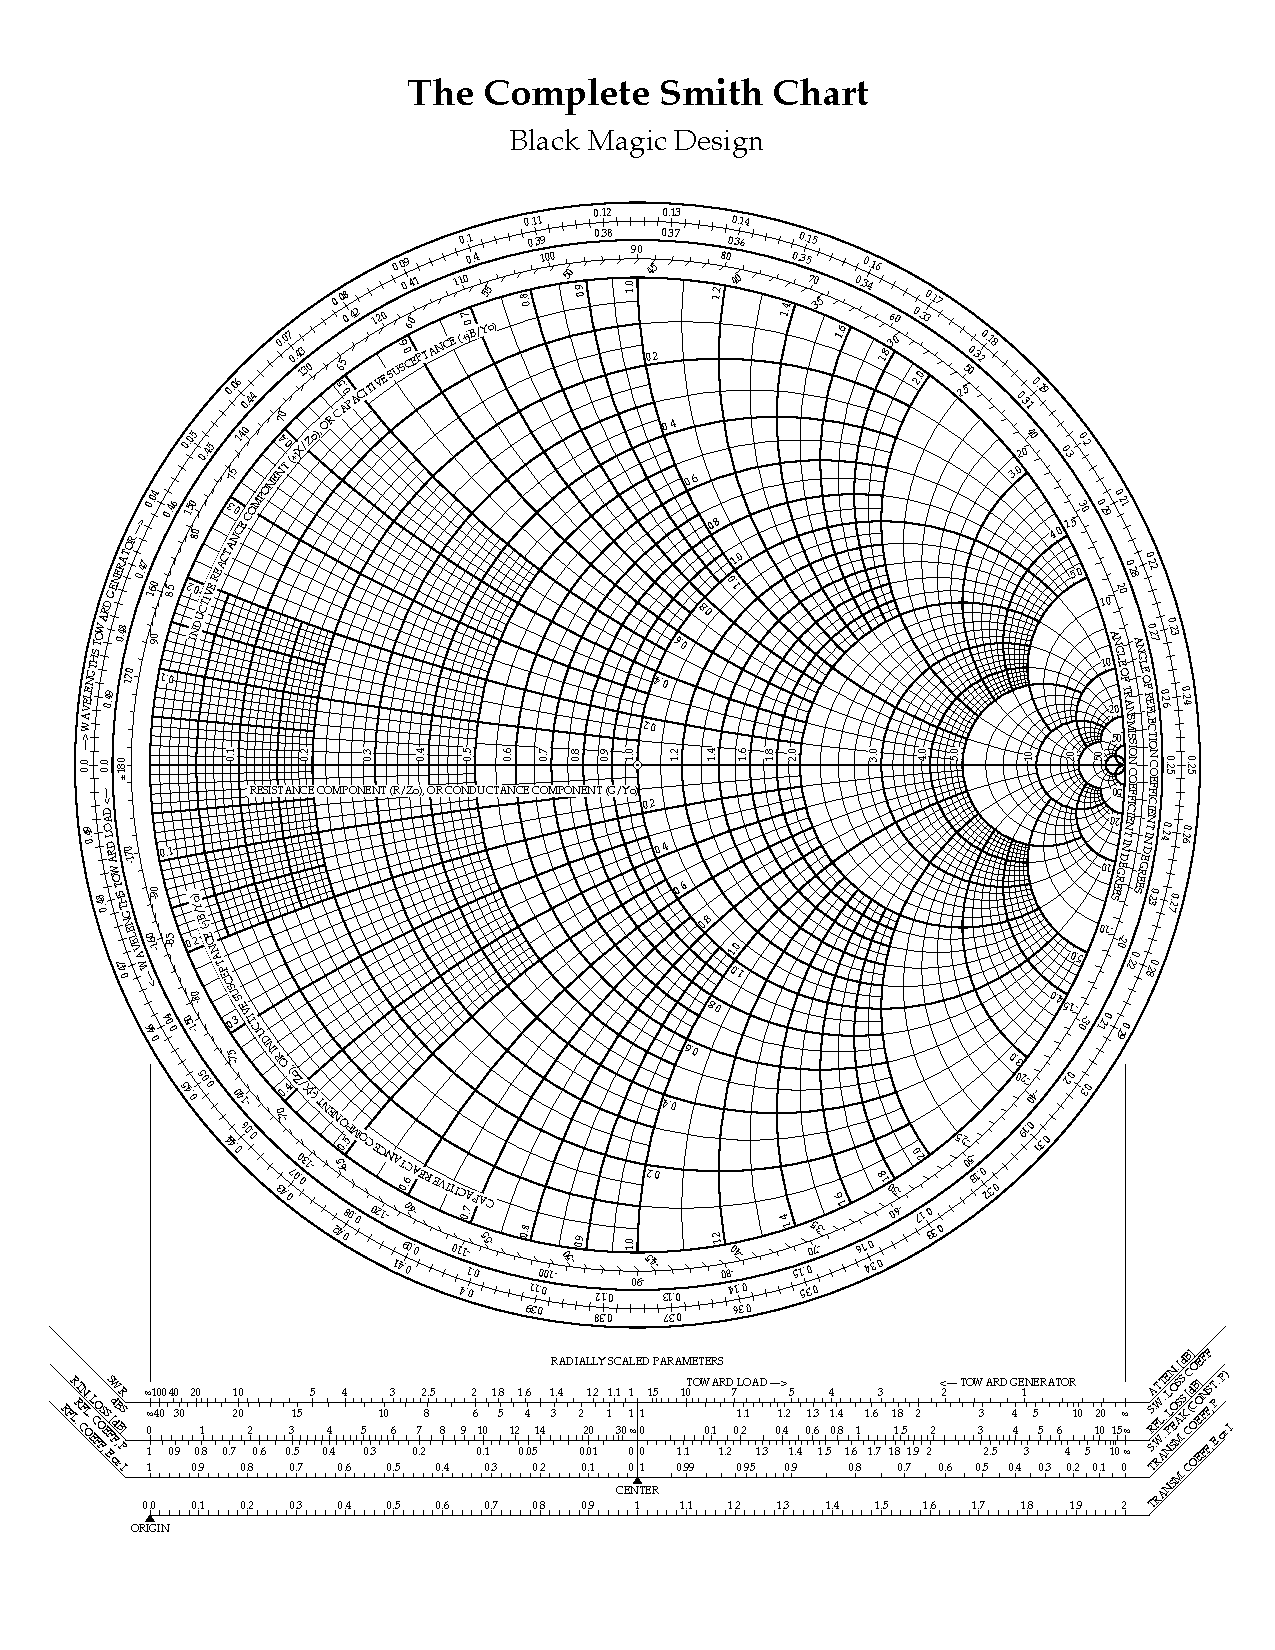
\includegraphics[scale=1.0,trim=1cm 2cm 1cm 3cm, clip]{./SmithChart}
\label{fig:SmithChart1}
\end{figure}
\newpage
\begin{figure}[H]
\centering
\vspace{4cm}
\hspace*{-1.6cm}
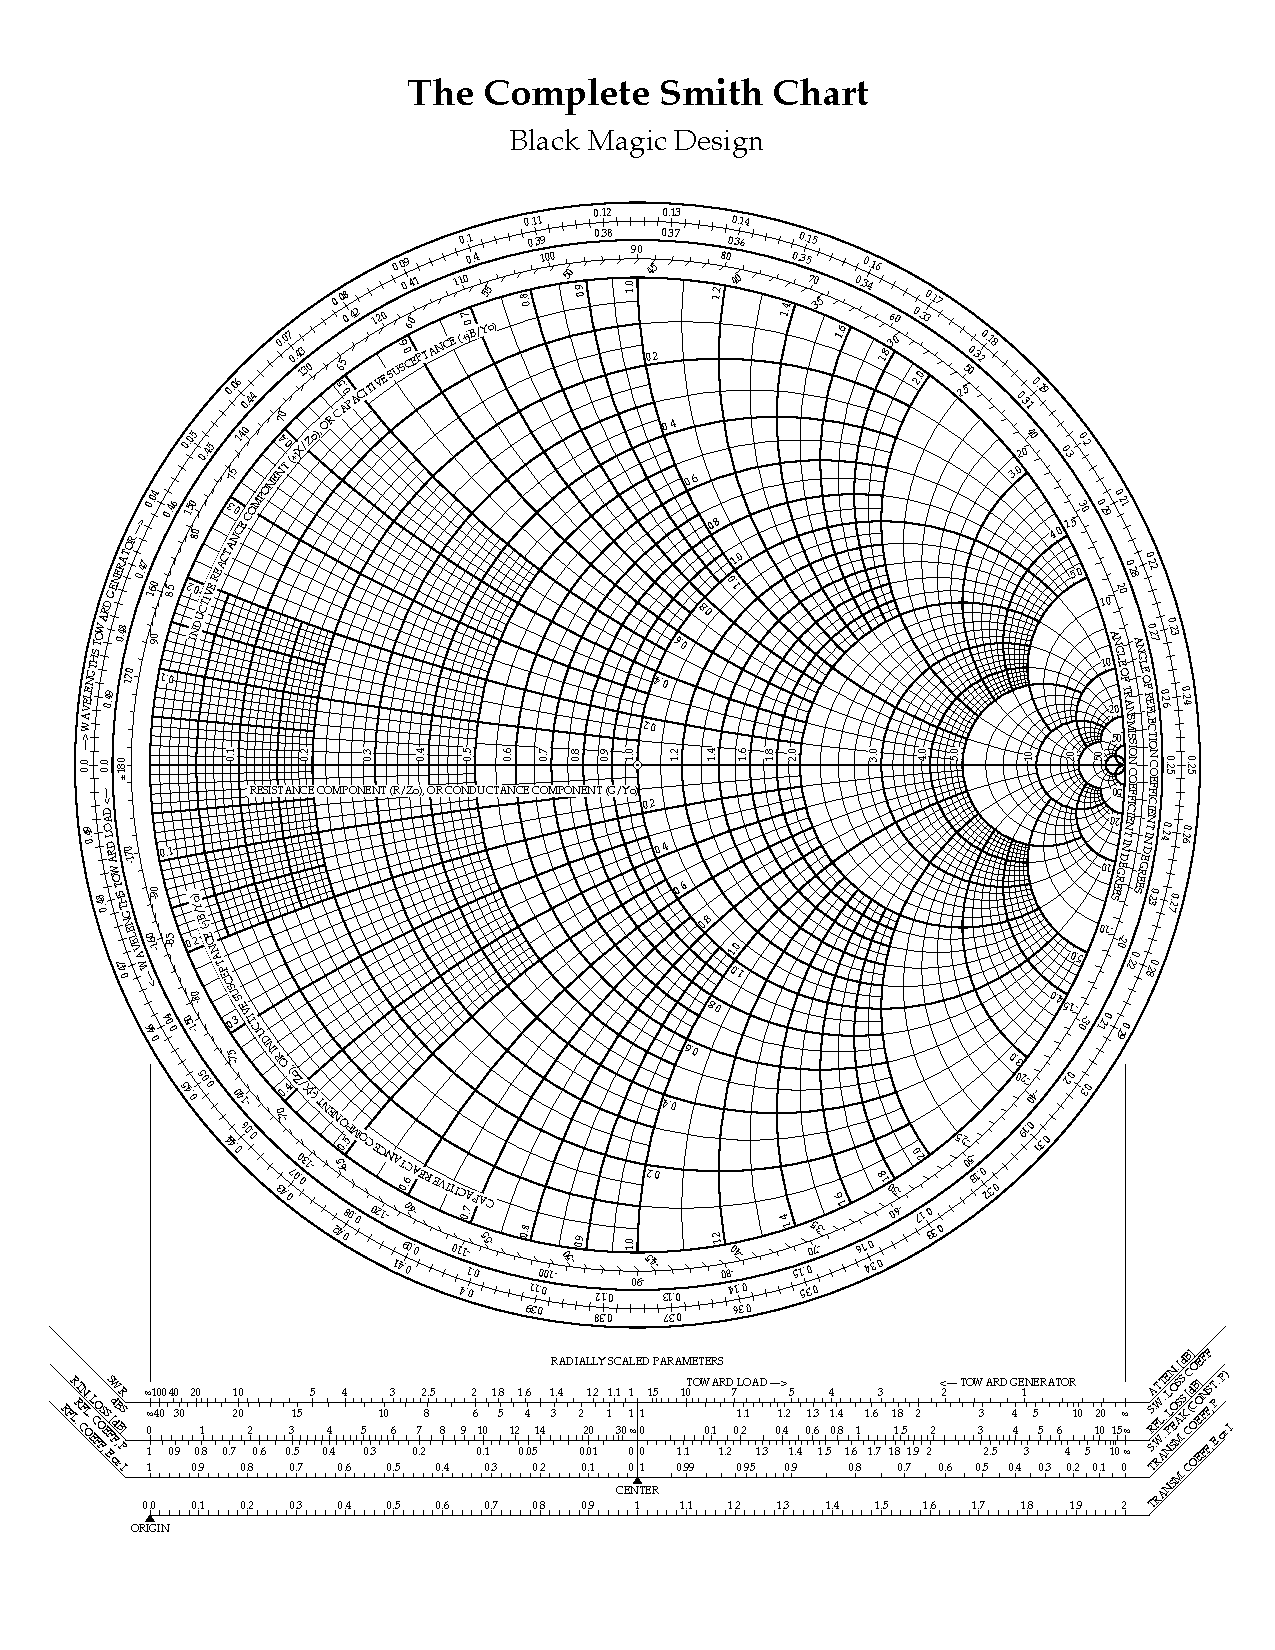
\includegraphics[scale=1.0,trim=1cm 2cm 1cm 3cm, clip]{./SmithChart}
\label{fig:SmithChart2}
\end{figure}
\newpage
\noindent\textbf{Question 3: \hfill \Qthree~marks}\\
A Teflon--filled rectangular waveguide is operating at 25 GHz. Waveguide dimensions are $a=1.07$ cm and $b=0.43$ cm. For Teflon: $\epsilon_r=2.08$ and $\mu_r=1$. The formula for cutoff frequency is $f_{c_{mn}}=\dfrac{ck_c}{2\pi\sqrt{\epsilon_r\mu_r}}$.
\begin{itemize}
\item[a.] Cutoff frequency ($f_c$) for $TE_{01}$ mode.
\item[b.] Components of electric and magnetic fields for $TE_{01}$ if $A=1$ and $B=1$.
\item[c.] Phase velocity.
\end{itemize}
\newpage~
\newpage
\begin{figure}[H]
\centering
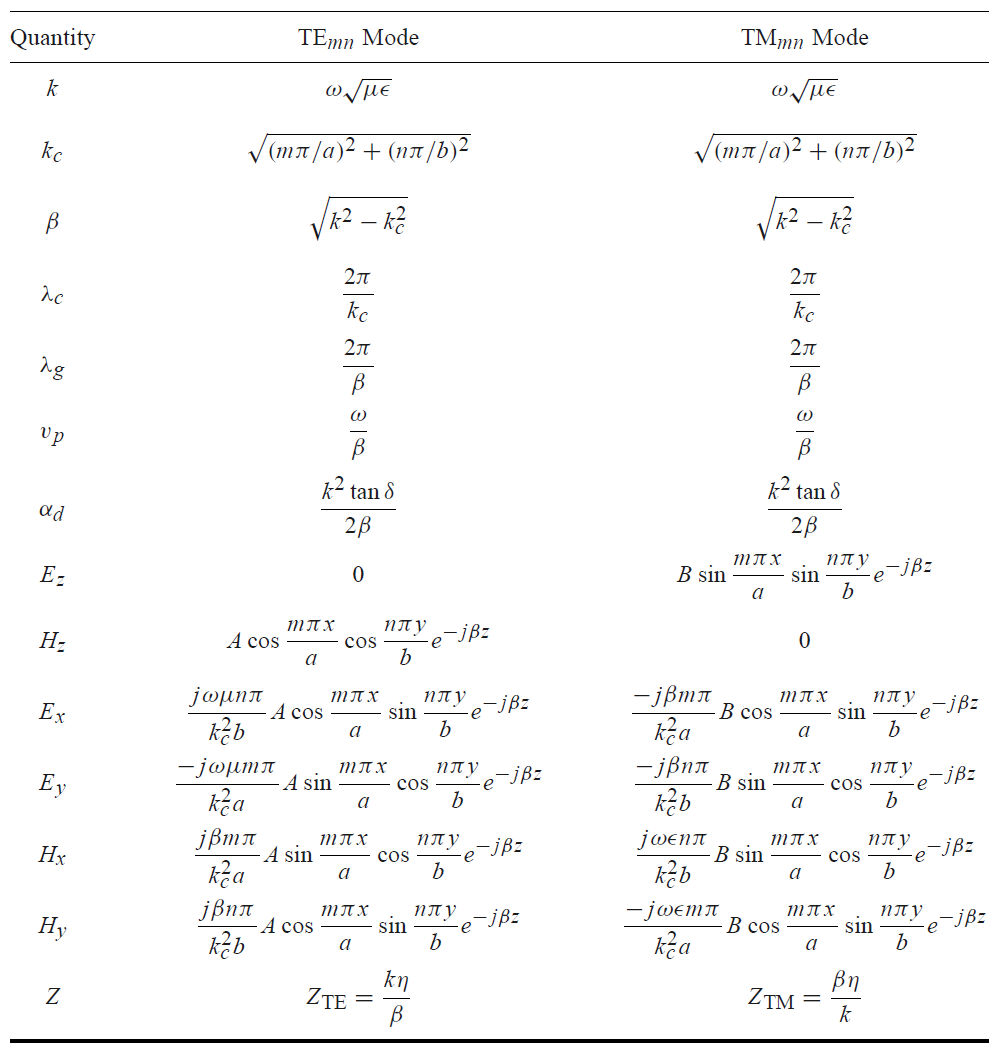
\includegraphics[width=\textwidth]{./WaveguideFormulas.png}
\label{fig:Waveguideformulas}
\end{figure}
\newpage
\noindent\textbf{Question 4: \hfill \Qfour~marks}\\
For the 2--port network shown in figure, find impedance, scattering and $ABCD$ parameters. Take $Z_0=2Z$.\\
\begin{flushleft}
$Z_{ij}=\dfrac{V_i}{I_j}\biggr\lvert_{I_k=0~for~k\neq j}$, $S_{ij}=\dfrac{V^-_i}{V^+_j}\biggr\lvert_{V^+_k=0~for~k\neq j}$\\[0.2cm]
$A=\dfrac{V_1}{V_2}\biggr\lvert_{I_2=0}$, $B=\dfrac{V_1}{I_2}\biggr\lvert_{V_2=0}$, $C=\dfrac{I_1}{V_2}\biggr\lvert_{I_2=0}$, $D=\dfrac{I_1}{I_2}\biggr\lvert_{V_2=0}$\\
\end{flushleft}
\begin{figure}[H]
\flushright
\vspace*{-4cm}
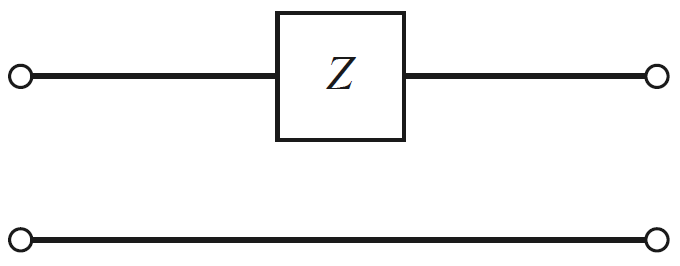
\includegraphics[width=0.3\textwidth]{./NetworkCircuit.png}
\label{fig:NetworkCircuit}
\end{figure}
\newpage~
\newpage~
\newpage
\noindent\textbf{Question 5: \hfill \Qfive~marks}\\
A BJT has the following scattering parameters at 1.0 GHz, with a 50 $\Omega$ reference impedance:\\$S_{11}=0.38\angle-158^0$, $S_{12}=0.11\angle54^0$, $S_{21}=3.5\angle80^0$ and $S_{22}=0.4\angle-43^0$. The source impedance is $Z_S=25~\Omega$ and load impedance is $Z_L=40~\Omega$. Draw the complete circuit diagram. Also compute the power gain, the available power gain and transducer power gain.\\
\begin{flushleft}
$\Gamma_{in}=S_{11}+\dfrac{S_{12}S_{21}\Gamma_L}{1-S_{22}\Gamma_L}$, $\Gamma_{out}=S_{22}+\dfrac{S_{12}S_{21}\Gamma_S}{1-S_{11}\Gamma_S}$\\[0.3cm]
$G=\dfrac{|S_{21}|^2(1-|\Gamma_L|^2)}{(1-|\Gamma_{in}|^2)|1-S_{22}\Gamma_L|^2}$\\[0.3cm]
$G_A=\dfrac{|S_{21}|^2(1-|\Gamma_S|^2)}{(1-|\Gamma_{out}|^2)|1-S_{11}\Gamma_S|^2}$\\[0.3cm]
$G_T=\dfrac{|S_{21}|^2(1-|\Gamma_S|^2)(1-|\Gamma_L|^2)}{|1-\Gamma_S\Gamma_{in}|^2|1-S_{22}\Gamma_L|^2}$\\
\end{flushleft}
\newpage~
\newpage~
\newpage~
\newpage
\begin{figure}[H]
\centering
\vspace{4cm}
\hspace*{-1.6cm}
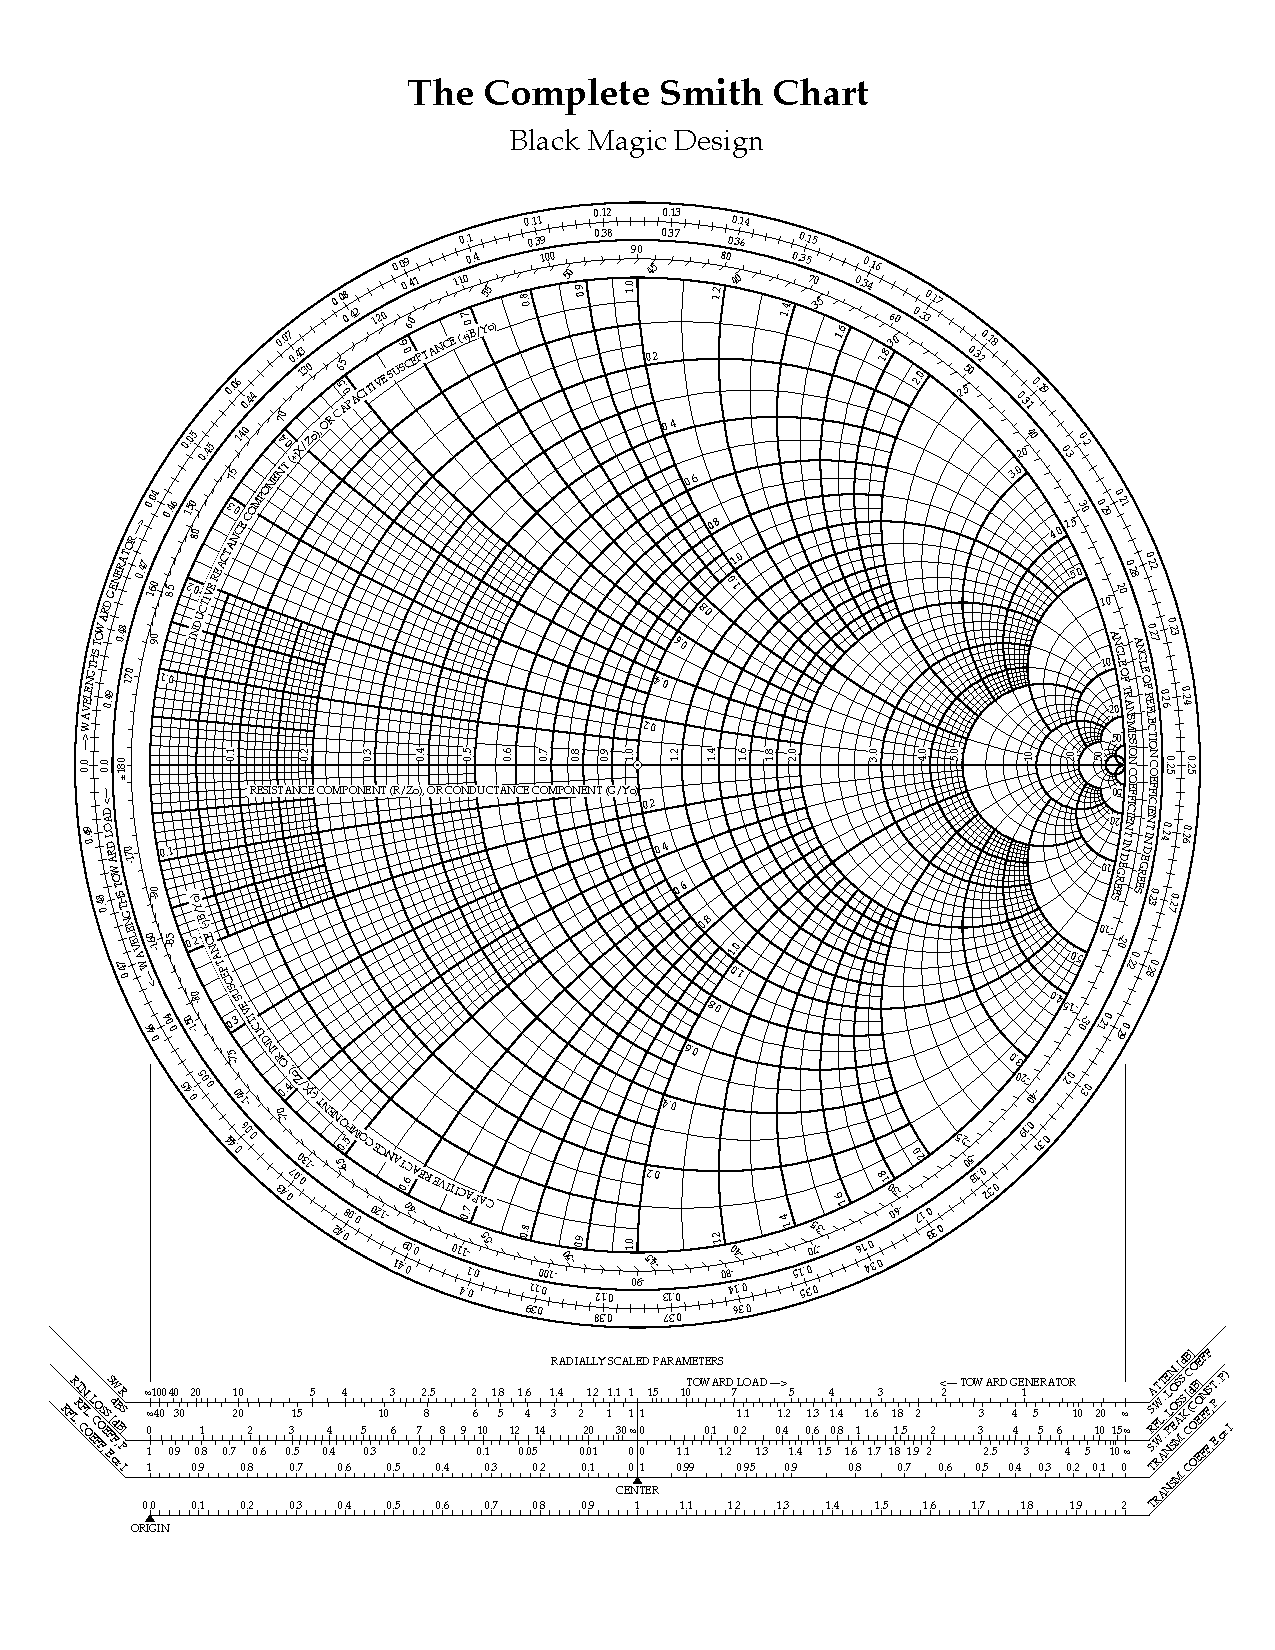
\includegraphics[scale=1.0,trim=1cm 2cm 1cm 3cm, clip]{./SmithChart}
\label{fig:SmithChart3}
\end{figure}
\end{document}